%!TEX root = ../BPlusTree-report.tex
\section{Problem Analysis}
\label{sec:ProblemAnalysis}
% Notes:
% Relevant constructs
%   - bplustree
%   - insert
%   - search 
%   - height
%   - deletion
% We want to prove:
%   - Insert works
%     - Inductive data types
%       - valid_bplus_tree
%       - appears_in_kvl
%       - appears_in_tree
%       - kvl_sorted
%     - Works under these assumptions...
%       -Valid bplustree
%       - Insertion preserves tree
%   - Search works
To implement B+ trees in Gallina, several different components have to be implemented. Most importantly, we must specify an inductive data type that describes a B+ tree, which can be seen in Fig. \ref{fig:inductive_data_type}.

\begin{figure}
\centering
\begin{coqdoccode}
\coqdockw{Inductive} \coqdocvar{bplustree} (\coqdocvar{b}: \coqdocvar{nat}) (\coqdocvar{X}:\coqdockw{Type}) : \coqdockw{Type} :=\coqdoceol
\coqdocindent{1.00em}
\ensuremath{|} \coqdocvar{bptLeaf} : \coqdocvar{list} (\coqdocvar{nat} \ensuremath{\times} \coqdocvar{X}) \ensuremath{\rightarrow} \coqdocvar{bplustree} \coqdocvar{b} \coqdocvar{X}\coqdoceol
\coqdocindent{1.00em}
\ensuremath{|} \coqdocvar{bptNode} : \coqdocvar{list} (\coqdocvar{nat} \ensuremath{\times} (\coqdocvar{bplustree} \coqdocvar{b} \coqdocvar{X})) \ensuremath{\rightarrow} \coqdocvar{bplustree} \coqdocvar{b} \coqdocvar{X}.\coqdoceol
\end{coqdoccode}
\caption{Inductive data type for B+ tree.}
\label{fig:inductive_data_type}
\end{figure}

\paragraph{}
This data type says that a $bplustree$ is parameterized by $b$, the order, and $X$, the type of the values in the tree. Further, a tree can be either a leaf or a node. A leaf is a list of key-value pairs of the types $nat$ and $X$, while a node is a list of key-pointer pairs with the types $nat$ and $bplustree$. Note that we use the term pointer in this report only for easy distinction between the two types of lists. There are, in fact, no pointers between trees in the internal Gallina representation. The ``pointers'' contained in nodes are actual values, just like the values in leaves, except the values in nodes can only be of the type $bplustree~bX$, i.e. a subtree with the same order and type as the parent tree.

\begin{figure}
 \centering
   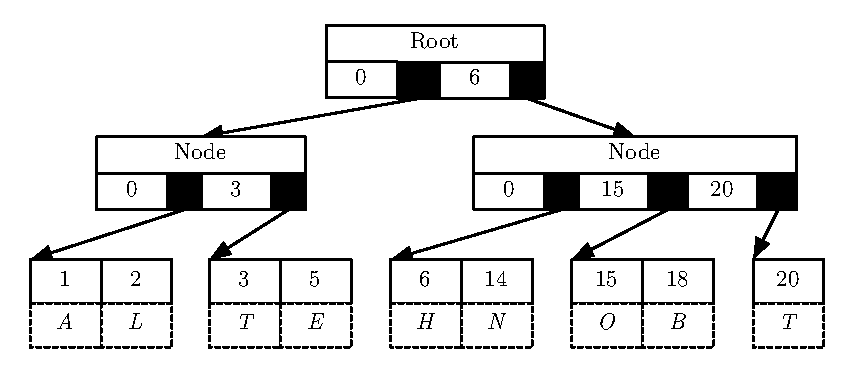
\includegraphics[width=90mm]{diagrams/BPlusTreeImpl.pdf}
 \caption{The same B+ tree as in Fig. \ref{fig:bplustree} but with our specific list implementation.}
 \label{fig:bplustreeImpl}
\end{figure}

\paragraph{}
Figure \ref{fig:bplustree} shows that for each node with $n$ keys there are $n+1$ pointers to sub trees. As it can be seen from both Fig. \ref{fig:inductive_data_type} and \ref{fig:bplustreeImpl} we have chosen to deal with this asymmetry by always having an explicit $0$ key in the beginning of each key-pointer list, such that a node with $n$ keys has $n$ pointers. This affects the order $b$ of the $bptNode$, as there can now be $b+1$ keys in each node before an overflow has to happen. Leaves are, of course, not affected and still can still only contain $b$ key-value pairs before it overflows.
\paragraph{}
A similar but trickier way to represent a node would be to have $n$ key-pointer pairs as well as a start pointer of the type $bplustree~b~X$. That would, however, give us unnecessary complexity both when writing our primary functions but also when proving theorems about these functions. Even though it is more strongly typed with such a definition we would always have to take care of a start pointer corner case when proving anything about our B+ trees. With our current solution we add a couple of assumptions to our notion of what a valid B+ tree is, to ensure the start pointer is properly handled. This will be explained in Section \ref{subsec:Valid_bplustree}.

\subsection{Time Complexity}
Even with an explicit start pointer, this functional implementation of B+ trees, which is an inherently imperative data structure, does have a short-coming when it comes to the asymptotic running time. A popular implementation of nodes and leaves entails representing the key-pointer and key-value pairs as an array, as it enables the fast binary search in the keys of a node. This implementation runs in $O(log(b))$ and makes the overall asymptotic complexity of B+ trees of $O(log(b)*h)$ possible for both Search and Insert operations. Using our data structure the running times of the these functions are limited to $O(h*b)$ as linear search of $b*2$ elements has to be performed in key lists for exactly $h$ nodes. 
\paragraph{}
Even though Gallina does not support arrays (as it is a pure functional language), there are a couple of ways to achieve a running time of $O(log(b))$ for the search through keys in nodes and leaves. The most obvious one is to represent the keys as a tree. This internal tree also has to be balanced and thus adds a lot extra complexity to the implementation. Implementing this internal tree structure was deemed out of scope. 
\paragraph{}
Another solution would be to use the Coq standard library map implementation, which has a concrete implementation that uses AVL trees\,\cite{fmapavl}. Using maps would require the emulation of arrays. In a node with $k$ keys there would be a mapping from a set of $k$ zero-indexed array keys to $k$ original keys. This is seen in Figure \ref{fig:bplustreeAVLImpl}, which is a representation of our example B+ tree with an AVL tree inside each node. A search for key 20 would do a search in the root's internal AVL tree, find a pointer to the right B+ tree node, do a search in the right B+ node's AVL tree to find that key 2 in the AVL tree has an end pointer to the leaf with value 20. 
\paragraph{}
Searching would be achievable in $O(log(b)*h)$ as search in the inner tree would have the asymptotic complexity of $O(log(b))$ as with binary search in an array. Insertion would have a less than optimal running time, as overflows in the tree would require the AVL tree to be traversed for two new half-trees to be constructed. Building these AVL trees would take $O(b*log(b))$ reducing the overall running time of insertion to $O(b*log(b)*h)$, which is worse than our current implementation.

\begin{figure}
 \centering
   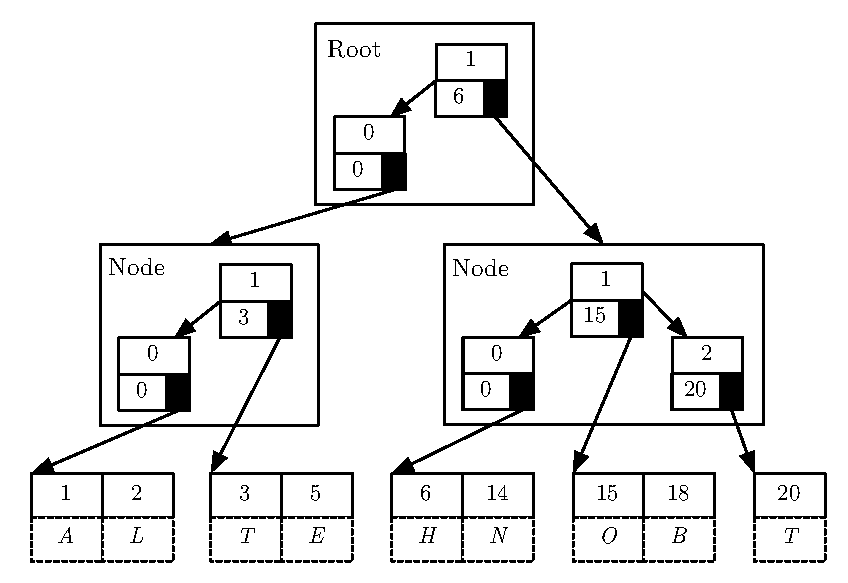
\includegraphics[width=90mm]{diagrams/BPlusTreeMapImpl.pdf}
 \caption{The same B+ tree as in Figure \ref{fig:bplustree} and \ref{fig:bplustreeImpl} but with an inner AVL tree to represent the node lists. Note that leaves are also represented as AVL trees even though it is not depicted here.}
 \label{fig:bplustreeAVLImpl}
\end{figure}

Apart from still not being an optimal solution, this implementation would add a large degree of complexity to our proofs, and since running time is not an objective of this project, it has been deemed out of scope to pursue such a B+ tree representation.


\subsection{Valid B+ tree}
\label{subsec:Valid_bplustree}
Although the inductive data type can represent a B+ tree, it says nothing about the validity of a tree. It is entirely possible to build B+ trees that break the constraints mentioned in the B+ trees background (Section \ref{subsec:Background_Bplus_tree}) using the $bplustree$ data type. To make statements about a B+ tree's validity, and to be sure that the trees we are working with are valid, we need a proposition that states what must hold for a B+ tree to be valid. This proposition is called $valid\_bplustree$, and can be seen in Fig. \ref{fig:inductive_valid_bplustree}. The proposition is inspired by Ramez et al. and altered to meet the implementation specific changes that we introduced in Section \ref{sec:ProblemAnalysis}\,\cite[pp. 652]{Elmasri1999}. 
\subsubsection{Valid Splits}
Before explaining this inductive data type we will first cover another inductive data type that $valid\_bplustree$ makes use of. This inductive data type is called $valid\_splits$ and guards the overall sorting of the B+ tree by ensuring that all keys of a sub tree are supposed to be in that sub tree.
\begin{itemize}
	\item The $valid_p$ proposition says that if the sub tree is between two keys $n1$ and $n2$ in the key-pointer list, then all keys of this sub tree must satisfy $n1 <= key < n2$. 
	\item In addition $valid_ep$ states that if the subtree is the last in the key-pointer list after key $n$ then all keys in the subtree must satisfy $n <= key$
\end{itemize} 

\begin{figure}

\begin{coqdoccode}
\coqdocnoindent
\coqdockw{Inductive} \coqdocvar{valid\_splits} (\coqdocvar{b}: \coqdocvar{nat}) (\coqdocvar{X}: \coqdockw{Type}) : \coqdocvar{list} (\coqdocvar{nat} \ensuremath{\times} \coqdocvar{bplustree} \coqdocvar{b} \coqdocvar{X}) \ensuremath{\rightarrow} \coqdockw{Prop} :=\coqdoceol
\coqdocindent{1.00em}
\ensuremath{|} \coqdocvar{valid\_p}  : \coqdockw{\ensuremath{\forall}} (\coqdocvar{t1} \coqdocvar{t2}: \coqdocvar{bplustree} \coqdocvar{b} \coqdocvar{X}) (\coqdocvar{n1} \coqdocvar{n2}: \coqdocvar{nat}) (\coqdocvar{l}: \coqdocvar{list} (\coqdocvar{nat} \ensuremath{\times} \coqdocvar{bplustree} \coqdocvar{b} \coqdocvar{X})),\coqdoceol
\coqdocindent{10.00em}
\coqdocvar{all} (\coqdocvar{between} \coqdocvar{n1} \coqdocvar{n2}) (\coqdocvar{keys} \coqdocvar{t1}) \ensuremath{\rightarrow}\coqdoceol
\coqdocindent{10.00em}
\coqdocvar{valid\_splits} \coqdocvar{b} \coqdocvar{X} ((\coqdocvar{n2}, \coqdocvar{t2})::\coqdocvar{l}) \ensuremath{\rightarrow}\coqdoceol
\coqdocindent{10.00em}
\coqdocvar{valid\_splits} \coqdocvar{b} \coqdocvar{X} ((\coqdocvar{n1}, \coqdocvar{t1})::(\coqdocvar{n2}, \coqdocvar{t2})::\coqdocvar{l})\coqdoceol
\coqdocindent{1.00em}
\ensuremath{|} \coqdocvar{valid\_ep} : \coqdockw{\ensuremath{\forall}} (\coqdocvar{t}: \coqdocvar{bplustree} \coqdocvar{b} \coqdocvar{X}) (\coqdocvar{n}: \coqdocvar{nat}),\coqdoceol
\coqdocindent{10.00em}
\coqdocvar{all} (\coqdocvar{above} \coqdocvar{n}) (\coqdocvar{keys} \coqdocvar{t}) \ensuremath{\rightarrow}\coqdoceol
\coqdocindent{10.00em}
\coqdocvar{valid\_splits} \coqdocvar{b} \coqdocvar{X} ([(\coqdocvar{n}, \coqdocvar{t})]).\coqdoceol
\end{coqdoccode}

\caption{Inductive data type for a valid splits in a B+ tree.}
\label{fig:inductive_valid_splits}
\end{figure}

\begin{figure}
\centering
\begin{coqdoccode}
\coqdockw{Inductive} \coqdocvar{valid\_bplustree} (\coqdocvar{b}: \coqdocvar{nat}) (\coqdocvar{X}: \coqdockw{Type}) : \coqdocvar{bplustree} \coqdocvar{b} \coqdocvar{X} \ensuremath{\rightarrow} \coqdockw{Prop} :=\coqdoceol
\coqdocindent{1.00em}
\ensuremath{|} \coqdocvar{root\_is\_a\_leaf}  : \coqdockw{\ensuremath{\forall}} (\coqdocvar{kvl}: \coqdocvar{list} (\coqdocvar{nat} \ensuremath{\times} \coqdocvar{X})), \coqdoceol
\coqdocindent{11.00em}
\coqdocvar{b} \ensuremath{\not=} 0 \ensuremath{\rightarrow}\coqdoceol
\coqdocindent{11.00em}
\coqdocvar{length} \coqdocvar{kvl} \ensuremath{\le} \coqdocvar{b} \ensuremath{\times} 2 \ensuremath{\rightarrow}\coqdoceol
\coqdocindent{11.00em}
\coqdocvar{kvl\_sorted} \coqdocvar{kvl} \ensuremath{\rightarrow}  \coqdoceol
\coqdocindent{11.00em}
\coqdocvar{valid\_bplustree} \coqdocvar{b} \coqdocvar{X} (\coqdocvar{bptLeaf} \coqdocvar{b} \coqdocvar{X} \coqdocvar{kvl})\coqdoceol
\coqdocindent{1.00em}
\ensuremath{|} \coqdocvar{valid\_root\_node} : \coqdockw{\ensuremath{\forall}} (\coqdocvar{kpl}: \coqdocvar{list} (\coqdocvar{nat} \ensuremath{\times} \coqdocvar{bplustree} \coqdocvar{b} \coqdocvar{X})),\coqdoceol
\coqdocindent{11.00em}
\coqdocvar{b} \ensuremath{\not=} 0 \ensuremath{\rightarrow} \coqdoceol
\coqdocindent{11.00em}
2 \ensuremath{\le} \coqdocvar{length} \coqdocvar{kpl} \ensuremath{\rightarrow} \coqdoceol
\coqdocindent{11.00em}
\coqdocvar{length} \coqdocvar{kpl} \ensuremath{\le} \coqdocvar{S} (\coqdocvar{b} \ensuremath{\times} 2) \ensuremath{\rightarrow}\coqdoceol
\coqdocindent{11.00em}
\coqdocvar{key\_at\_index} 0 \coqdocvar{kpl} = \coqdocvar{Some} 0 \ensuremath{\rightarrow} \coqdoceol
\coqdocindent{11.00em}
\coqdocvar{all\_values} (\coqdocvar{bplustree} \coqdocvar{b} \coqdocvar{X}) (\coqdocvar{valid\_sub\_bplustree} \coqdocvar{b} \coqdocvar{X}) \coqdocvar{kpl} \ensuremath{\rightarrow}\coqdoceol
\coqdocindent{11.00em}
\coqdocvar{all\_values\_eq\_prop} (\coqdocvar{bplustree} \coqdocvar{b} \coqdocvar{X}) \coqdocvar{equal\_height} \coqdocvar{kpl} \ensuremath{\rightarrow}\coqdoceol
\coqdocindent{11.00em}
\coqdocvar{kvl\_sorted} \coqdocvar{kpl} \ensuremath{\rightarrow}  \coqdoceol
\coqdocindent{11.00em}
\coqdocvar{valid\_splits} \coqdocvar{b} \coqdocvar{X} \coqdocvar{kpl} \ensuremath{\rightarrow}\coqdoceol
\coqdocindent{11.00em}
\coqdocvar{valid\_bplustree} \coqdocvar{b} \coqdocvar{X} (\coqdocvar{bptNode} \coqdocvar{b} \coqdocvar{X} \coqdocvar{kpl})   \coqdoceol
\end{coqdoccode}
\caption{Inductive data type for a valid B+ tree.}
\label{fig:inductive_valid_bplustree}
\end{figure}

\subsubsection{Sorting the Individual Lists}
\label{sec:Kvl_sorted}
While $valid\_splits$ argue about the overall sorting of the tree, we need to reason about the individual sorting of the key-pointer and key-value pairs within the nodes and leafs. For this reason we have introduced the inductive proposition $kvl\_sorted$, which we have reproduced in Fig. \ref{fig:kvl_sorted}.

\begin{figure}
  \begin{coqdoccode}
  \coqdocnoindent
  \coqdockw{Inductive} \coqdocvar{kvl\_sorted} \{\coqdocvar{X}: \coqdockw{Type}\}: \coqdocvar{list} (\coqdocvar{nat} \ensuremath{\times} \coqdocvar{X}) \ensuremath{\rightarrow} \coqdockw{Prop} :=\coqdoceol
  \coqdocindent{1.00em}
  \ensuremath{|}
  \coqdocvar{kvl\_sorted\_0}: \coqdocvar{kvl\_sorted} []\coqdoceol
  \coqdocindent{1.00em}
  \ensuremath{|} \coqdocvar{kvl\_sorted\_1}: \coqdockw{\ensuremath{\forall}} (\coqdocvar{n}: \coqdocvar{nat}) (\coqdocvar{x}: \coqdocvar{X}), \coqdoceol
  \coqdocindent{8.00em}
  \coqdocvar{kvl\_sorted} [(\coqdocvar{n}, \coqdocvar{x})]\coqdoceol
  \coqdocindent{1.00em}
  \ensuremath{|} \coqdocvar{kvl\_sorted\_cons}: \coqdockw{\ensuremath{\forall}} (\coqdocvar{n1} \coqdocvar{n2}: \coqdocvar{nat}) (\coqdocvar{x1} \coqdocvar{x2}: \coqdocvar{X}) (\coqdocvar{lst}: \coqdocvar{list} (\coqdocvar{nat} \ensuremath{\times} \coqdocvar{X})), \coqdoceol
  \coqdocindent{8.00em}
  \coqdocvar{kvl\_sorted} ((\coqdocvar{n2},\coqdocvar{x2})::\coqdocvar{lst}) \ensuremath{\rightarrow} \coqdoceol
  \coqdocindent{8.00em}
  \coqdocvar{blt\_nat} \coqdocvar{n1} \coqdocvar{n2} = \coqdocvar{true} \ensuremath{\rightarrow}\coqdoceol
  \coqdocindent{8.00em}
  \coqdocvar{kvl\_sorted} ((\coqdocvar{n1},\coqdocvar{x1})::(\coqdocvar{n2},\coqdocvar{x2})::\coqdocvar{lst}).\coqdoceol
  \end{coqdoccode}
  \caption{The $kvl\_sorted$ proposition we use to argue about the sorting of lists.}
  \label{fig:kvl_sorted}
\end{figure}

The rules about sorting is very straight forward: A empty list and the list containing exactly one element is always sorted. If you have a sorted list, you can add a smaller element to the beginning of it, and it will remain sorted.

\subsubsection{The Main Proposition}
This proposition is only valid when examining the root of a tree, as there are different constraints for subtrees (See Section \ref{subsec:Background_Bplus_tree}). $valid\_bplustree$ has two cases, the first holds when the root of the B+ tree is a leaf, and the second holds when the root is a node. The various properties that must hold are explained below.

\paragraph{Root is a leaf}
The following must hold for a root leaf to be a valid B+ tree:
\label{valid_root_is_a_leaf}
\begin{itemize}
\item $b \neq 0$ --- The order must not be 0. Since we are working with natural numbers, this means $b > 0$.
\item $length\ kvl \leq b \times 2 $ --- The leaf must have at most $2b$ elements.
\item $kvl\_sorted\ kvl$ --- The keys in the leaf must be sorted.
\end{itemize}

\paragraph{Root is a node}
The following must hold for a root node to be a valid B+ tree:
\label{valid_root_is_a_node}
\begin{itemize}
\item $b \neq 0$ --- The order must not be 0.
\item $2 \leq length\ kpl$ and $length\ kpl \leq S\ (b \times 2)$ --- These satisfy the conditions for order stated in Section \ref{subsec:Background_Bplus_tree}.
\item $key\_at\_index\ 0\ kpl = Some\ 0$ --- As mentioned above, we must know that the first key is always 0. This assures that this is the case.
\item $all\_values (bplustree\ b\ X)\ (valid\_sub\_bplustree\ b\ X)\ kpl$ --- All the values stored in the node (the pointers) must be valid subtrees. As mentioned in Section \ref{subsec:Background_Bplus_tree}, the constraints for the root are slightly different. The constraints for internal leaves and nodes will be covered below.
\item $all\_values\_eq\_prop (bplustree\ b\ X)\ equal\_height\ kpl$ --- All subtrees must have the same height.
\item $kvl\_sorted\ kpl$ --- The keys in the node must be sorted.
\item $valid\_splits\ b \ X\ kpl$ --- See Valid Splits section above.
\end{itemize}

Since $valid\_bplustree$ only holds for the root leaf or node, a different proposition is needed for non-root leaves and nodes, or subtrees. This is implemented in the $valid\_sub\_bplustree$ proposition.\todo{Insert in appendix and insert a reference here} In the interest of brevity, only the differences will be listed here:

\paragraph{Non-root leaf}
\begin{itemize}
\item $b \leq length\ kvl$ --- The number of key-value pairs in the leaf must be at least $b$.
\end{itemize}

\paragraph{Non-root node}
\begin{itemize}
\item $2 \leq length\ kpl$ changed to $S\ b \leq length\ kpl$ --- The number of key-pointer pairs must be at least $b+1$.
\end{itemize}

\paragraph{}
With the $bplustree$ data type we can start implementing the search and insert functions, and $valid\_bplustree$ gives us the assumptions that are needed for proving facts about these functions.

\subsection{Search}
\label{subsec:search}
Our implementation of search does not stray far from the prototypical version described in the background (Section \ref{sec:Background}). It is implemented through 3 functions: $search'$, $find\_subtree$, and $search\_leaf$. 

\paragraph{}
$insert$ and $search$ are both recursive functions, recursing over a decreasing parameter $counter$. The reason for introducing this parameter is to serve as a recursion terminator. Since a key requirement for recursive Coq functions is that they must contain a decreasing argument, we introduced this notion of a counter that will decrease by one every time we descend down a subtree. Because our inductive type for B+ trees consists of a nesting of two inductive data types that are not mutually recursive, Coq is unable to tell that a $bplustree$ is decreasing when it is used as an argument. If the counter ever reaches $0$, the recursion stops. This means that should the counter ever reach $0$ before we have descended all the way down the tree, a wrong result will be given. To ensure this never happens, we always initialize the counter to the height of the tree\todo{Jesper: You must show the code!}.

\paragraph{}
The reason why initializing the counter to the height of the tree will guarantee that our counter will never reach $0$ before our $insert'$ implementation has descended all the way down to a leaf is simple. Our implementation of $height$ simply counts the number of steps it takes to descend down the leftmost child in every node until it reaches a leaf. Our $valid\_bplustree$ proposition captures the balancing nature of B+ trees, so if $height$ is called on a valid B+ tree, the returned height is the number of steps from the root to any leaf in the tree. So regardless of which leaf is inserted into, we know we can descend that far down the tree in $counter$ steps. Because our implementation of $insert'$ only decreases the counter by one every time it recursively calls itself with a subtree, we have a invariant where the counter will always be exactly equal to the height of the tree it is currently processing. This invariant is a key aspect to constructing induction proofs on our B+ trees, as our implementation doesn't have a data type that is inductively defined over the height of the tree.

\paragraph{}
A key part of both insertion and searching in our implementation is the function $find\_subtree$. This function, when given a list of key-pointer pairs, and a search-key, will identify the key-pointer pair whose range contains the search-key. The pointer in the identified key-pointer pair is the subtree that, in a valid B+ tree, must contain the search-key if the tree contains the key.

\paragraph{}
The main function that performs search is $search'$, that as mentioned above is recursively defined over a natural number counter. It uses $find\_subtree$ to identify which subtree to recurse into, and when it reaches a leaf it calls $search\_leaf$. $search\_leaf$ performs a simple linear search through the key-value pairs to identify if the search-key exists within the tree, and if so, returns the associated value. To ensure that the counter is always initialized to the height of the tree to search, we have added a definition of $search$ that simply calls $search'$ with $counter = height~tree$.

\subsection{Insert}
The $insert$ function calls the $insert'$ function to insert into a tree. First $insert'$ recurses down through $counter$ layers to find the insertion point, after which it handles overflow, if any should occur, on the way back up through the recursion layers. The function $insert'$ never increases the height of the tree but lets $insert$ handle the case where the root node overflows. In this case $insert$ will split the former root node into two sub nodes and connect these to a new root. This case obviously increases the height of the tree by $1$ and keeps the tree balanced. Effectively, this means the invariant described in Section \ref{subsec:search} still holds for $insert'$, as the height of the balanced tree is always equal to the $counter$ variable, which the $insert'$ function is decreasing on.

\paragraph{}
Out of the three central $insert$, $insert'$ and $insert\_leaf$ functions, the most significant is $insert'$. It uses $find\_subtree$ to figure out which subtree it should recurse into and $insert\_node$ to handle overflowing subtrees. Where $insert'$ handles overflowing leaves, $insert\_node$ takes care of overflowing (non-root) nodes.

\subsection{Elements of a Complete Proof of Correctness}
\label{sec:ElementsOfACompleteProof}
For insertion and search, a formal verification of the implementations would\todo{Jesper: Would? Don't you do it?} entail a combination of three different (but related) main proofs.

\subsubsection{Insert Search Works}
Whenever we insert into a tree with insert, we must be able to find it again afterwards. This is true even in the case where the key already exists and we have to overwrite the value. The proposition looks the following way: $search\ k\ (insert\ k\ v\ t) = Some\ v$, and it can be found in InsertSearchWorksProofs.v.

\subsubsection{Insert Preserves Validity}
It is, however, not enough to just show that an inserted element is retrievable. It says nothing about the validity of the tree and thus the insertion function could easily leave the tree unbalanced or otherwise invalid. With the definition of a valid B+ tree from Section \ref{subsec:Valid_bplustree}, we can define the following proposition that must hold: $valid\_bplustree\ b\ X\ tree\ \rightarrow valid\_bplustree\ b\ X\ (insert\ k\ v\ tree)$. It can be found in InsertPreservesProofs.v.

\subsubsection{Insert Preserves Elements}
As a final guard we must ensure that insert does not throw away elements from the initial tree or inserts other elements. A flawed implementation of insert, designed to circumvent the two above-mentioned proofs, could just return a leaf with the inserted key-value pair for all trees. By using an in-order traversal of the tree, together with a simple insertion into the sorted list it produces, we can ensure that no elements are lost, and that only the $(k, v)$ pair is inserted. In its simplest form it is structured the following way: $insert\_into\_list\ k\ v\ (inorder\ t) = inorder\ (insert\ k\ v\ t)$. See InsertPreservesElements.v for the full specification of the proof.

\subsubsection{Scope and Proof Limitations}
Proving these three main theorems in Coq is an immense task. As a consequence, we have chosen to focus on the most central one, which is the InsertSearchWorks proof, as it is the most heavily depended upon of the three, as it only holds if all the primary functions are correct.

\paragraph{}
As mentioned above, only proving InsertSearchWorks leaves the possibility for a incorrect implementation of insert that just throws away the initial tree and returns a leaf with the inserted element. We will let it be up to the reader to verify\todo{Jesper: This is an awesome task as you say. Don't push work you haven't done on the reader, but write something slightly weaker about trust.} that our insertion function is not implemented that way, and so we list InsertPreservesElements as future work. Conversely, the assumption that the insertion function ensures that the validity of the tree is preserved is much more difficult to manually verify. Not having proved InsertPreserves is a central admission in the proof of InsertSearchWorks, as the search function assumes that the input tree is valid. Given the fact that we currently do not ensure that the tree is valid after insertion, we cannot prove that the input tree handed to the search function (in our InsertSearchWorks proof) is actually valid. InsertPreserves is classified as future work as well.
